\section{Analyse avec la NMF et K-means}
Comme mentionné précédemment, deux méthodes d'analyse ont été utilisées pour identifier les thèmes dans les romans de Zola : la NMF (Non-negative Matrix Factorization) et K-means. Cette section présente ces deux méthodes et expose les choix retenus pour leur application au corpus préparé.

\subsection{La méthode NMF}

La NMF est une technique de réduction de dimensionnalité qui permet d'extraire des thèmes à partir d'un corpus de textes. Elle fonctionne en factorisant la matrice terme-document en deux matrices non négatives : une matrice de thèmes et une matrice de poids. La matrice de thèmes contient les mots les plus représentatifs de chaque thème, tandis que la matrice de poids indique l'importance de chaque thème dans chaque document ou paquet de phrases.

La présentation commence par la NMF, avant d'aborder le clustering par K-means comme méthode complémentaire.

Après la préparation du corpus, la segmentation en paquets de phrases et la lemmatisation des textes, l'étape suivante consiste à appliquer une méthode de modélisation thématique. L'objectif est d'identifier automatiquement les grands thèmes présents dans les romans de Zola, à partir des termes les plus représentatifs de chaque segment textuel.

Dans cette analyse, la méthode retenue est la NMF, pour \textit{Non-negative Matrix Factorization}. Cette méthode permet de décomposer une matrice terme-document en deux matrices plus simples : une matrice associant les segments de texte aux topics, et une matrice associant les topics aux termes les plus caractéristiques. La NMF est particulièrement adaptée à ce type d'analyse, car elle produit des résultats relativement interprétables : chaque topic peut être compris comme un ensemble de mots fortement associés entre eux.

\subsubsection{Création de la matrice terme-document}

La première étape consiste à transformer les textes lemmatisés en une représentation numérique exploitable par le modèle. Pour cela, une matrice terme-document a été construite à l'aide d'une pondération TF-IDF\footnote{Utilisée via la bibliothèque \texttt{scikit-learn}.}. Cette méthode permet de donner un poids plus important aux termes caractéristiques d'un segment, tout en réduisant l'influence des mots trop fréquents dans l'ensemble du corpus.

Les paramètres \texttt{min\_df} et \texttt{max\_df} jouent un rôle important dans la qualité de la matrice obtenue. Le paramètre \texttt{min\_df=3} permet d'exclure les mots qui apparaissent dans moins de trois segments. Ces mots sont généralement trop rares pour contribuer efficacement à l'identification de thèmes récurrents. À l'inverse, le paramètre \texttt{max\_df=0.8} exclut les termes présents dans plus de 80 \% des segments, car ils sont trop fréquents pour être réellement discriminants\footnote{Le vectoriseur est disponible en annexe.}.

Ce choix relève d'un arbitrage méthodologique. Plusieurs combinaisons ont été testées, puis évaluées à partir de la qualité des mots conservés et de la cohérence des premiers topics obtenus. L'objectif n'était donc pas seulement de réduire la taille de la matrice, mais surtout de conserver les termes les plus utiles pour l'analyse thématique. La matrice finale sert ensuite de base à l'application du modèle NMF.

\subsubsection{Choix du nombre de topics}

Le choix du nombre de topics constitue une étape importante dans une analyse par NMF. Un nombre trop faible de topics risque de produire des catégories trop générales, dans lesquelles plusieurs thèmes distincts se trouvent regroupés. À l'inverse, un nombre trop élevé peut conduire à une fragmentation excessive des résultats, avec des topics trop proches les uns des autres ou difficiles à interpréter.

Afin d'orienter ce choix, une méthode du coude a d'abord été utilisée\footnote{Code visible en annexe.}. Cette méthode consiste à entraîner plusieurs modèles NMF avec différents nombres de topics, puis à observer l'évolution de l'erreur de reconstruction. L'objectif est d'identifier un éventuel seuil à partir duquel l'ajout de nouveaux topics n'améliore plus fortement la qualité de reconstruction du modèle.

\begin{figure}[H]
    \centering
    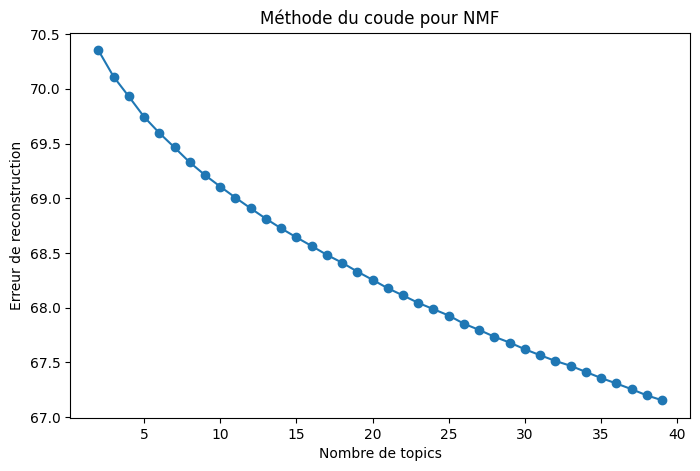
\includegraphics[width=0.8\textwidth]{images/chapitre_1/methodologie/coude_2_40.png}
    \caption{Méthode du coude pour le choix du nombre de topics dans la NMF, entre 2 et 40 topics}
    \label{fig:methode_du_coude_nmf_2_40}
\end{figure}

La première visualisation présente l'évolution de l'erreur de reconstruction pour un nombre de topics compris entre 2 et 40. On observe une diminution régulière de l'erreur lorsque le nombre de topics augmente. Cette baisse est attendue : plus le modèle dispose de topics, plus il peut reconstruire finement la matrice terme-document. Cependant, la courbe ne présente pas de rupture nette permettant d'identifier un coude évident. Le critère quantitatif ne suffit donc pas, à lui seul, à déterminer un nombre optimal de topics.

Une seconde visualisation a été produite en resserrant l'observation sur une zone plus restreinte, comprise entre 20 et 39 topics. Ce zoom permet d'examiner plus précisément la partie de la courbe dans laquelle plusieurs valeurs candidates pouvaient être envisagées.

\begin{figure}[H]
    \centering
    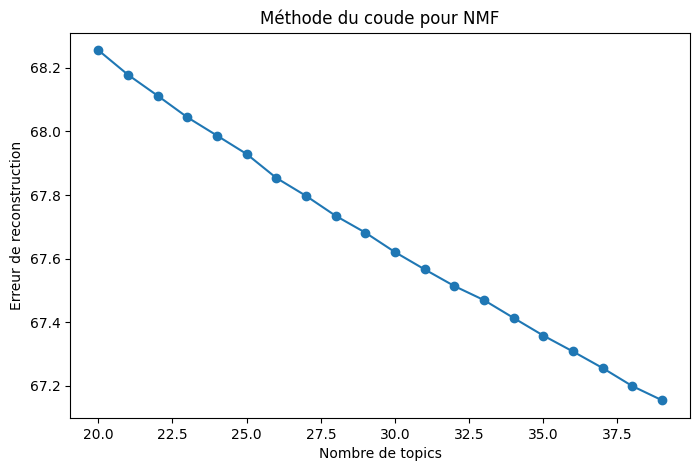
\includegraphics[width=0.8\textwidth]{images/chapitre_1/methodologie/methode_du_coude_nmf.png}
    \caption{Méthode du coude pour le choix du nombre de topics dans la NMF, entre 20 et 39 topics}
    \label{fig:methode_du_coude_nmf_20_39}
\end{figure}

Ce second graphique confirme l'absence de seuil clairement marqué. L'erreur de reconstruction continue de diminuer de manière progressive, sans stabilisation brutale ni changement de pente suffisamment net pour imposer une valeur unique. Le choix du nombre de topics ne peut donc pas reposer uniquement sur la méthode du coude.

Le choix final a ainsi été complété par une analyse qualitative des résultats. Plusieurs valeurs ont été testées, notamment 10, 15, 20, 30 et 35 topics. Les modèles obtenus ont été comparés à partir des mots caractéristiques de chaque topic, de leur cohérence interne et de leur capacité à correspondre à des thèmes interprétables dans l'œuvre de Zola. Dans cette perspective, le choix de 29 topics a été retenu comme un compromis entre précision, lisibilité et stabilité interprétative.

Ce choix a également été mis en relation avec l'analyse par K-means. Le nombre de clusters retenu pour K-means a été fixé à 29 afin de permettre une comparaison directe entre les deux méthodes. Cette seconde approche ne sert pas à prouver définitivement que 29 est le nombre optimal de topics, mais elle permet de vérifier si une structuration thématique comparable apparaît lorsque les segments sont regroupés selon une logique différente. Autrement dit, K-means joue ici un rôle de validation complémentaire : si certains motifs apparaissent à la fois dans les topics NMF et dans les clusters K-means, cela renforce leur pertinence pour l'analyse du corpus.
\subsubsection{Paramétrage du modèle NMF}

Après plusieurs essais, le modèle final a été construit avec 29 topics. Cette valeur a été retenue, car elle permettait d'obtenir un niveau de détail suffisant, sans produire une fragmentation trop importante des thèmes ni introduire trop de bruit. Les topics obtenus correspondent à des ensembles thématiques distincts, comme le monde ouvrier, la religion, la famille, la finance, la guerre, le commerce, la médecine ou encore l'espace domestique, comme nous le verrons dans la section consacrée aux résultats.

Le paramètre \texttt{n\_components=29} correspond au nombre de topics recherchés. Le paramètre \texttt{random\_state=42} permet d'assurer la reproductibilité des résultats. L'initialisation \texttt{nndsvda}\footnote{L'initialisation \texttt{nndsvda} correspond à une variante de NNDSVD dans laquelle les zéros sont remplacés par la moyenne de la matrice. Voir la documentation de \texttt{scikit-learn}.} est adaptée à la NMF, car elle fournit une initialisation stable à partir de la structure de la matrice. Le solveur \texttt{cd}, pour \textit{coordinate descent}, est utilisé pour optimiser la factorisation.

La matrice \texttt{W} contient les poids des topics pour chaque segment du corpus. Autrement dit, elle indique dans quelle mesure chaque segment est associé à chacun des 29 topics. La matrice \texttt{H}, quant à elle, contient les poids des mots pour chaque topic. Elle permet donc d'identifier les termes les plus représentatifs de chaque thème.

\subsubsection{Limites de l’approche}

L’utilisation de la NMF présente plusieurs avantages, notamment sa lisibilité et sa capacité à produire des topics relativement interprétables. Cependant, cette méthode comporte aussi des limites. Le choix du nombre de topics reste en partie subjectif, surtout lorsque la méthode du coude ne permet pas d’identifier une valeur optimale claire. Dans cette analyse, le choix de 29 topics repose donc sur un compromis entre précision, lisibilité et cohérence interprétative. La validation humaine des résultats est donc essentielle pour s'assurer que les topics produits correspondent à des thèmes réels et pertinents dans l'œuvre de Zola.

De plus, les noms attribués aux topics résultent d’une interprétation humaine. Deux personnes pourraient parfois proposer des intitulés légèrement différents pour un même groupe de mots. Il est donc important de considérer ces noms comme des outils d’analyse, et non comme des catégories fixes ou définitives. Cette subjectivité ne remet pas en cause la validité de l’analyse, mais elle souligne l’importance d’une approche critique et réflexive dans l’interprétation des résultats.

Enfin, les résultats dépendent fortement des choix effectués en amont : nettoyage du texte, lemmatisation, liste de mots à exclure, taille des segments, paramètres du vectoriseur et nombre de topics. La modélisation thématique ne doit donc pas être comprise comme une méthode entièrement automatique, mais comme un processus exploratoire qui combine traitement statistique et interprétation qualitative avec validation humaine à chaque étape.

\subsubsection{Bilan méthodologique}

Cette étape de modélisation par NMF permet d'obtenir une première cartographie thématique du corpus romanesque de Zola. Elle fournit une base quantitative pour observer des régularités lexicales qui seront ensuite interprétées dans la section consacrée aux résultats.

La NMF constitue donc un outil pertinent pour explorer les thèmes récurrents dans un corpus littéraire volumineux. Elle ne remplace pas l’analyse littéraire, mais elle permet de faire apparaître des régularités lexicales et thématiques qui peuvent ensuite être interprétées plus finement. Dans le cadre de cette étude, elle sert à établir une base quantitative pour l’analyse des thèmes présents dans les romans de Zola.

\subsection{La méthode K-means}

Après l'application de la NMF, une seconde méthode a été utilisée afin de compléter l'analyse thématique du corpus : le clustering par K-means. Contrairement à la NMF, qui cherche à décomposer la matrice terme-document en topics latents, K-means vise à regrouper les segments textuels en ensembles homogènes à partir de leur proximité lexicale. L'objectif n'est donc pas exactement le même : la NMF permet d'identifier des thèmes sous forme de combinaisons de mots, tandis que K-means permet de regrouper les paquets de phrases qui présentent des profils lexicaux similaires.

Cette seconde méthode a été utilisée comme un outil complémentaire de comparaison et de validation. Elle permet de vérifier si les regroupements produits par la NMF correspondent également à des ensembles cohérents lorsque l'on applique une méthode de clustering non supervisée. Dans le cadre de cette analyse, chaque paquet de phrases constitue une unité d'observation, représentée numériquement par une matrice TF-IDF. Les clusters obtenus correspondent donc à des groupes de segments partageant des termes caractéristiques.

\subsubsection{Préparation de la matrice TF-IDF}

Comme pour la NMF, la première étape consiste à transformer les textes lemmatisés en une représentation numérique. La matrice utilisée pour le K-means est construite à partir des segments lemmatisés du corpus. Le même type de vectorisation TF-IDF et les mêmes paramètres ont été conservés afin d'assurer une cohérence méthodologique entre les deux approches\footnote{Voir la section consacrée à la préparation de la matrice terme-document dans l'approche NMF.}.

Ce choix permet de travailler sur une matrice plus lisible et plus pertinente pour le clustering. Le but n'est pas seulement de réduire le nombre de dimensions, mais aussi de conserver les mots qui participent réellement à la différenciation des segments. Cette étape est essentielle, car la qualité des clusters dépend directement de la qualité de la représentation vectorielle utilisée.

\subsubsection{Recherche du nombre de clusters}

Le choix du nombre de clusters est une étape centrale dans l'utilisation de K-means. Un nombre trop faible de clusters risque de produire des groupes trop généraux, dans lesquels plusieurs thèmes différents seraient mélangés. À l'inverse, un nombre trop élevé peut produire des groupes trop fragmentés, difficiles à interpréter ou très proches les uns des autres.

Afin d'orienter ce choix, plusieurs valeurs de \texttt{k} ont été testées. Pour chaque valeur comprise entre 2 et 40, un modèle K-means a été entraîné, puis évalué à l'aide du score de silhouette\footnote{Peter J. Rousseeuw, « Silhouettes: A graphical aid to the interpretation and validation of cluster analysis », \textit{Journal of Computational and Applied Mathematics}, vol. 20, 1er novembre 1987, p. 53--65.}.

Ce score mesure la qualité de la séparation entre les clusters : plus il est élevé, plus les segments sont proches des éléments de leur propre cluster et éloignés des autres groupes.

Une visualisation des scores de silhouette a ensuite été produite afin d'observer l'évolution de la qualité du clustering selon le nombre de clusters.

\begin{figure}[H]
    \centering
    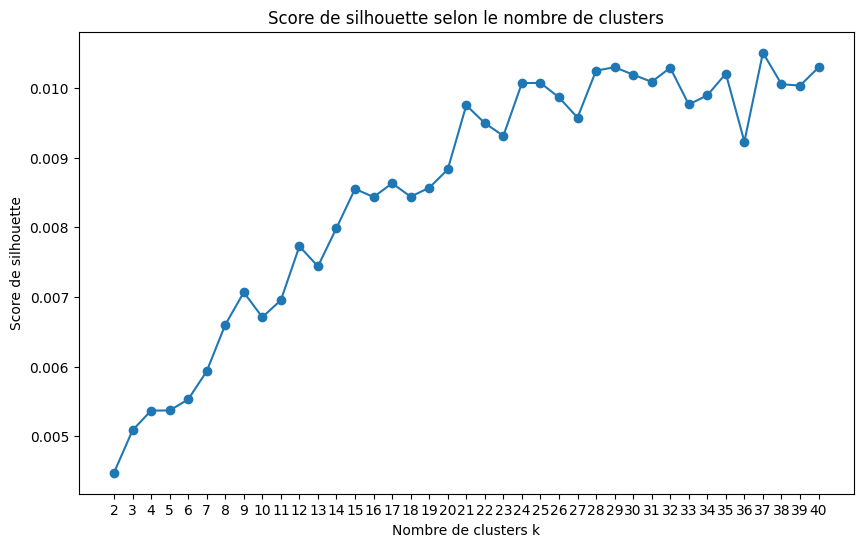
\includegraphics[width=0.8\textwidth]{images/chapitre_1/methodologie/silhouette.png}
    \caption{Évolution du score de silhouette en fonction du nombre de clusters dans K-means}
    \label{fig:silhouette_kmeans}
\end{figure}

Dans cette analyse, le score de silhouette fournit une indication quantitative, mais il ne suffit pas à lui seul à déterminer le nombre de clusters à retenir. Comme pour la NMF, le choix final repose donc sur un compromis entre indicateurs statistiques, lisibilité des résultats et cohérence interprétative. Le nombre de 29 clusters a été retenu afin de permettre une comparaison directe avec les 29 topics issus de la NMF, tout en conservant un niveau de détail suffisant pour distinguer les principaux motifs thématiques du corpus. De plus, le score de silhouette reste relativement stable autour de cette valeur, ce qui indique que les clusters obtenus sont globalement cohérents.

\subsubsection{Entraînement du modèle K-means}

Le modèle K-means final a été entraîné avec 29 clusters. Le paramètre \texttt{random\_state=42} permet d'assurer la reproductibilité des résultats, tandis que le paramètre \texttt{n\_init=10} indique que l'algorithme est lancé plusieurs fois avec des initialisations différentes afin de retenir la meilleure solution.

Chaque segment du corpus reçoit ainsi un numéro de cluster après l'entraînement du modèle. L'ajout de \texttt{+ 1} permet de numéroter les clusters à partir de 1 plutôt qu'à partir de 0, ce qui rend les résultats plus lisibles dans les tableaux et les visualisations. Chaque paquet de phrases est donc associé à un groupe thématique déterminé par sa proximité avec les autres segments du corpus.


\subsubsection{Limites de l'approche par K-means}

L'utilisation de K-means présente plusieurs limites qu'il faut prendre en compte. Tout d'abord, la méthode impose une appartenance unique de chaque segment à un cluster. Or, dans un texte littéraire, un même passage peut contenir plusieurs thèmes simultanément. Un segment peut par exemple associer la famille, l'argent et la souffrance sociale, mais K-means l'attribue malgré tout à un seul groupe. Cette contrainte rend la méthode moins souple que la NMF pour représenter la complexité thématique des textes.

Ensuite, le choix du nombre de clusters reste en partie subjectif. Le score de silhouette fournit une indication utile, mais il ne suffit pas toujours à identifier une valeur optimale. Dans cette analyse, le choix de 29 clusters repose donc sur un arbitrage méthodologique : il permet de conserver un niveau de détail comparable à celui de la NMF, tout en produisant des catégories suffisamment interprétables.

Une autre limite concerne la sensibilité de K-means à la représentation vectorielle. Les clusters dépendent fortement de la matrice TF-IDF, des choix de lemmatisation, de la liste de mots exclus et des paramètres \texttt{min\_df} et \texttt{max\_df}. Une modification de ces choix peut modifier la structure des clusters obtenus, comme cela peut également être le cas avec la NMF. Les résultats doivent donc être compris comme une cartographie exploratoire du corpus, et non comme une classification définitive.

Enfin, comme pour la NMF, la nomination des clusters repose sur une interprétation humaine. Les intitulés attribués aux clusters et aux grandes familles de motifs sont construits à partir des mots les plus représentatifs et de l'observation des segments. Cette étape qualitative est nécessaire pour donner du sens aux résultats, mais elle introduit aussi une part de subjectivité.

\subsubsection{Bilan méthodologique}

L'ajout d'une classification hiérarchique sur les centres des clusters permet également d'organiser les résultats en grandes familles de motifs. Cette étape rend l'analyse plus lisible, car elle permet de passer de 29 clusters détaillés à cinq ensembles thématiques plus généraux, qui seront interprétés dans la section consacrée aux résultats.


Après la présentation des deux méthodes, la section suivante expose les principaux résultats obtenus, d'abord pour la NMF, puis pour K-means.